%
% Tesi D.S.I. - modello preso da
% Stanford University PhD thesis style -- modifications to the report style
%
%%%%%%%%%%%%%%%%%%%%%%%%%%%%%%%%%%%%%%%%%%%%%%%%%%%%%%%%%
%
%
\makeatletter
\let\my@xfloat\@xfloat
\makeatother
\documentclass[a4paper,12pt]{report}
%    \renewcommand{\baselinestretch}{1.6}      % interline spacing
%
% \includeonly{}
%
%			PREAMBOLO
%
\usepackage[a4paper]{geometry}
\usepackage{amssymb,amsmath,amsthm}
\usepackage{graphicx}
\graphicspath{{./img/}}
\usepackage{url}
\usepackage{hyperref}
\usepackage{epsfig}
\usepackage[italian]{babel}
\usepackage{setspace}
\usepackage{tesi}
\makeatletter
\def\@xfloat#1[#2]{
	\my@xfloat#1[#2]%
	\def\baselinestretch{1}%
	\@normalsize \normalsize
}
\makeatother


% per le accentate
\usepackage[utf8]{inputenc}
%
\newtheorem{myteor}{Teorema}[section]
%
\newenvironment{teor}{\begin{myteor}\sl}{\end{myteor}}
%
%
%			TITOLO
%
\begin{document}
\begin{center}

\includegraphics[width=\textwidth]{Logo.jpg}
\title{Realizzazione di una soluzione IAC (Infrastructure As Code) che consenta il rilascio di un'infrastruttura per ambiti DevOps}
\end{center}
\author{\textbf{Roberto Antoniello}}
\dept{Corso di Laurea in Informatica} 
\anno{2022-2023}
\matricola{\textbf{875693}}
\relatore{Prof. Valentina Ciriani}
\correlatore{Mario Petrella}

\beforepreface

\afterpreface
% 
% 
% 
\chapter{Introduzione}
\section{IAC: definizione e vantaggi}
La metodologia IAC(Infrastructure As Code), in italiano "infrastruttura come codice", è una strategia che punta a gestire l'intero ciclo di vita di un'infrastruttura mediante codice. Quindi non c'è bisogno di configurazione hardware fisica o strumenti interattivi esterni, è sufficiente uno o più linguaggi dichiarativi o di scripting e compilare correttamente dei file di definizione.\cite{iacdef} \\ 
In questo modo è molto più semplice e rapido modificare o eseguire miglioramenti al sistema senza dover ripensare completamente la struttura o stravolgerne le componenti. \\
Come vedremo nei successivi paragrafi, la potenza di alcune delle tecnologie trattate lungo lo sviluppo di questo progetto risiede proprio nel fatto di poter essere gestite direttamente tramite codice.\\
In questo capitolo introduttivo saranno descritti gli obiettivi prefissati per questo progetto, le fasi principali che sono state svolte e una breve descrizione delle tecnologie utilizzate. \\
In questo modo sarà più immediato richiamare alcuni concetti che useremo nei capitoli successivi.
\section{Obiettivi del progetto}
Gli obiettivi principali prefissati per questo progetto di tirocinio sono stati i seguenti:
\begin{enumerate}
\item \textit{Acquisire competenze in ambito DevOps.}
\item \textit{Acquisire conoscenze sul ciclo di vita di un'infrastruttura.}
\item \textit{Costruire un'infrastruttura in grado di essere rilasciata attraverso il cloud e sulla quale fosse possibile rilasciare applicazioni basate su microservizi.}
\end{enumerate}
\subsection{Dal metodo tradizionale all'approccio DevOps}
DevOps è una metodologia che punta a ridurre in modo considerevole i tempi di rilascio di nuovo software incorporando nello stesso di team di sviluppo le competenze necessarie per costruire l'infrastruttura adatta al rilascio del software grazie ai concetti di container, microservizi e cloud computing.\\
Tradizionalmente il processo di rilascio avveniva più lentamente nell'arco di mesi. Il team di sviluppo doveva coordinarsi con gli altri team per le diverse fasi dello sviluppo. Oggi invece con lo sviluppo DevOps si possono eseguire tutte le fasi senza dover aspettare un team separato, garantendo che il tempo di rilascio delle modifiche del software possa avvenire con frequenza oraria o anche meno, oltre ad essere continuativo e automatico.\\
Un'ulteriore progresso in questo tipo di approcci è il DevSecOps, una strategia che va a integrare anche la sicurezza e il testing nel CI(Continuous Integration) e CD(Continuous Deployment). \\La difficoltà che sorge nel DevSecOps è la risoluzione dei problemi legati alla sicurezza internamente al team di sviluppo, poichè gli sviluppatori devono prima acquisire le competenze necessarie per risolvere questo tipo di problemi.
\subsection{Ciclo di vita dell'infrastruttura}
Si intende in tal senso che l'obiettivo specifico fosse di comprendere l'intero ciclo a partire dall'analisi dei requisiti fino ad arrivare alla progettazione e implementazione finale del sistema.
\section{Fasi principali svolte}
Le principali fasi svolte durante il progetto di tirocinio sono state le seguenti:
\begin{enumerate}
\item \textit{Studio delle tecnologie coinvolte.} \\
Durante questa fase sono state approcciate diverse tecnologie per la prima volta. Vi è stato un primo apprendimento teorico dei concetti che ruotavano attorno al funzionamento di questi strumenti, mentre successivamente tali concetti sono stati applicati in maniera pratica eseguendo diversi test.
\item \textit{Progettazione dell'infrastruttura.}
\item \textit{Implementazione del sistema.}
\end{enumerate}

\section{Tecnologie utilizzate}
\begin{figure}[h]
	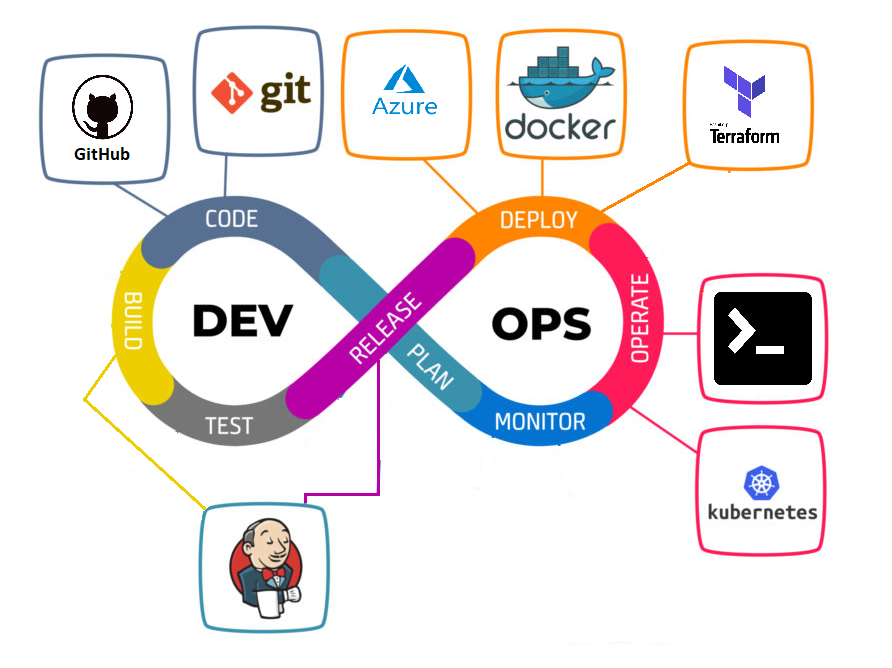
\includegraphics[width=0.6\textwidth]{tech_used}
    \caption{The DevOps infinity loop(ogni tecnologia utilizzata nel proprio settore) \cite{devopsloop}}
    \label{fig:tech_used}
\end{figure}


\chapter{Studio delle tecnologie coinvolte e analisi dei requisiti}
\section{Tecnologie}
\subsection{Kubernetes}
\subsection{Azure}
\subsection{Terraform}
\subsection{Jenkins}
\section{Requisiti}
\subsection{collegamenti tra le tecnologie}

\chapter{Progettazione dell'infrastruttura}
\section{Casi d'uso}
\section{Definizione dell'infrastruttura}
\subsection{Ulteriori dettagli progettuali}

\chapter{Implementazione in funzione dei disegni progettuali}
\section{Codice Terraform e pipeline dedicata}
\subsection{Definizione via codice}
\subsection{pipeline per la gestione delle modifiche}
\section{Sviluppo pipeline per il rilascio dei micro servizi e modifica di puntamenti nel sorgente}
\subsection{Definizione delle pipeline}
\subsection{Modifica nel codice sorgente}

\chapter{Conclusioni: risultati raggiunti e possibili miglioramenti}
\section{risultati raggiunti al termine}
\section{miglioramenti}

%
%			BIBLIOGRAFIA
%
\begin{thebibliography}{00}
%
\bibitem{iacdef}
Wikipedia, Infrastructure As Code. \url{https://it.wikipedia.org/wiki/Infrastructure_as_Code}
\bibitem{devopsloop}
TechTarget, Demystify the DevOps process, step by step, 2023.  \url{https://www.techtarget.com/searchitoperations/tip/Demystify-the-DevOps-process-step-by-step}

%
%
\end{thebibliography}
% 
\end{document}


 
